% !TEX program = xelatex
% !TEX encoding = UTF-8 Unicode
% !Mode:: "TeX:UTF-8"

\documentclass{resume}
\usepackage{graphicx}
\usepackage{tabu}
\usepackage{multirow}
\usepackage{progressbar}
\usepackage{zh_CN-Adobefonts_external} % Simplified Chinese Support using external fonts (./fonts/zh_CN-Adobe/)
%\usepackage{zh_CN-Adobefonts_internal} % Simplified Chinese Support using system fonts
\usepackage{linespacing_fix} % disable extra space before next section
\usepackage{cite}

\begin{document}
\pagenumbering{gobble} % suppress displaying page number

\Large{
  \begin{tabu}{ c l r }
   \multirow{5}{1in}{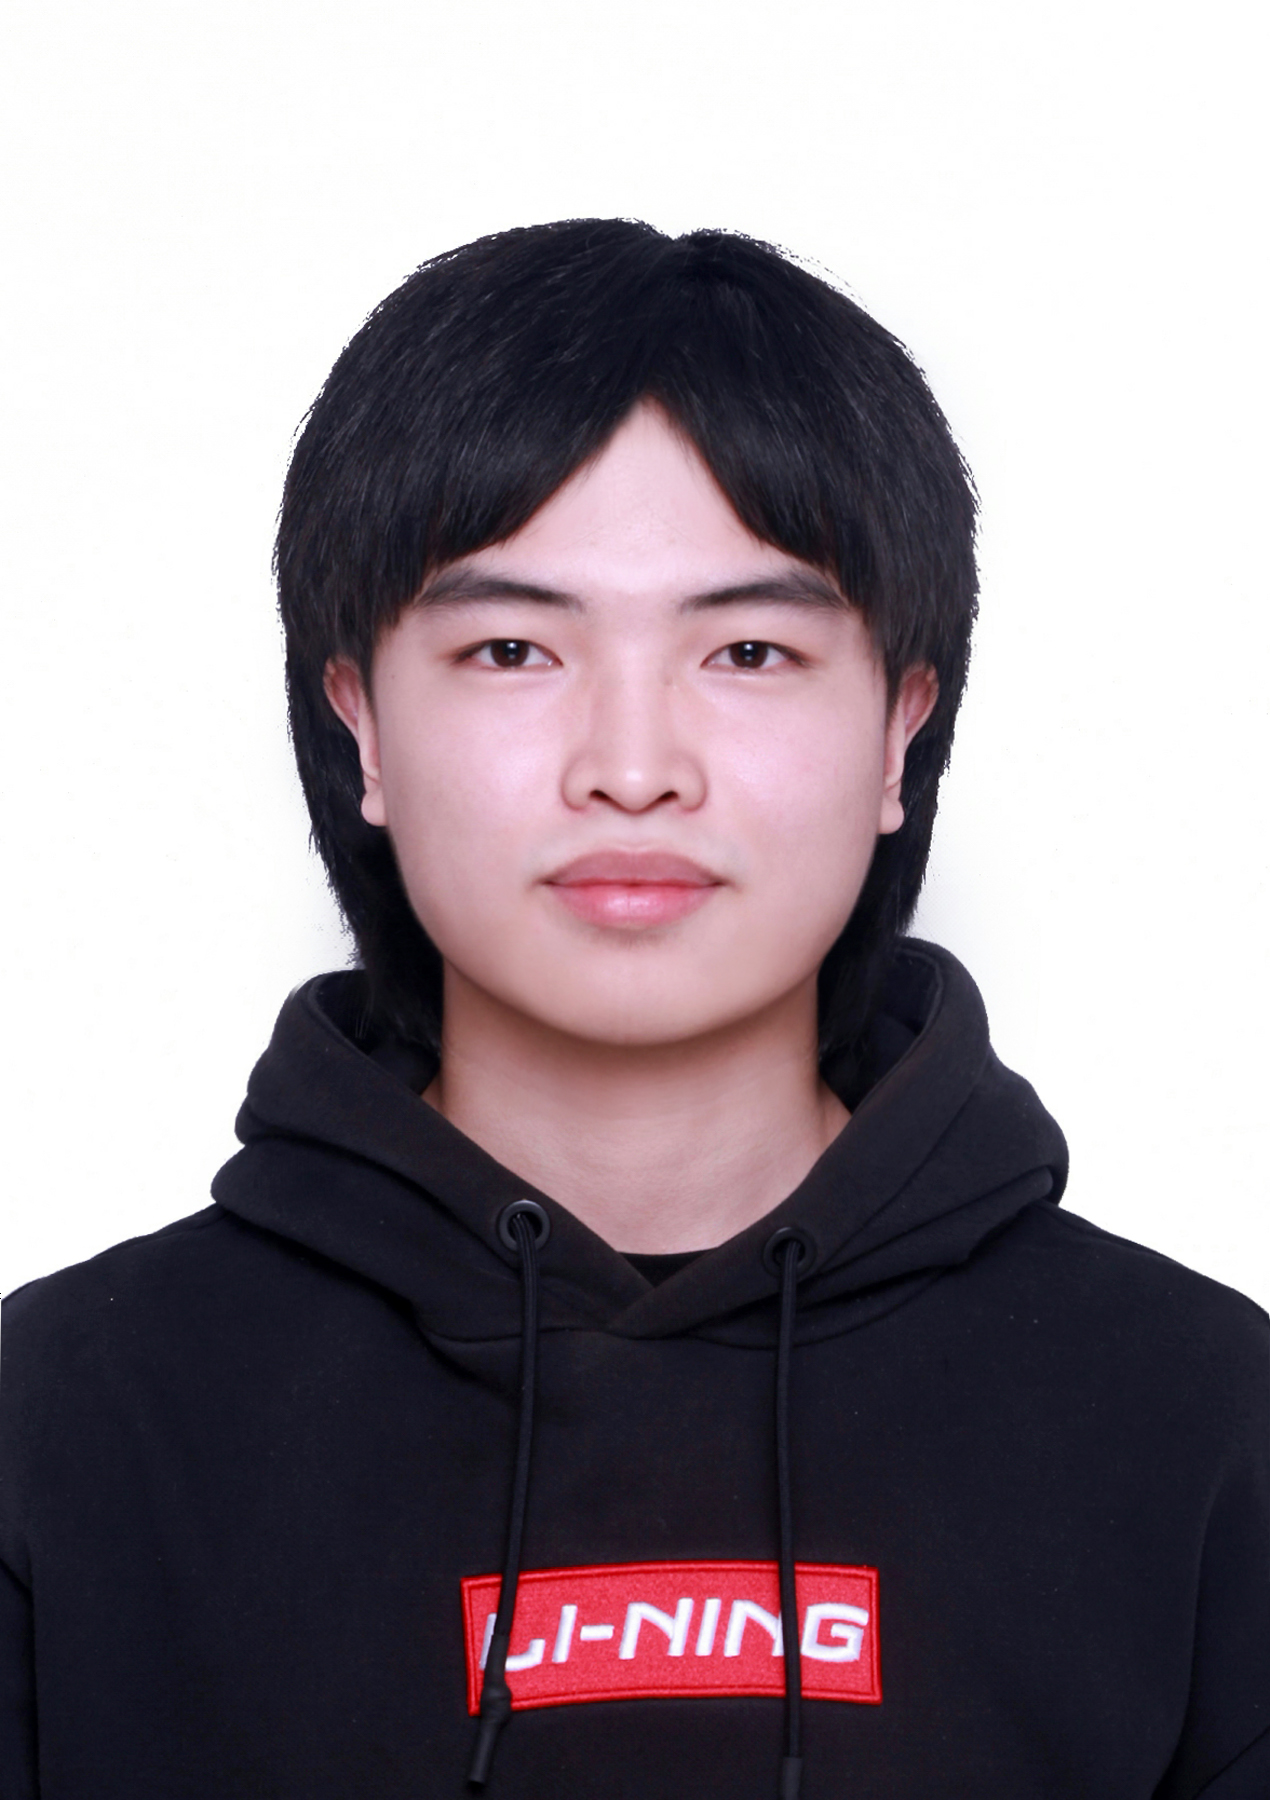
\includegraphics[width=0.88in]{avatar}} & \scshape{段启阳}  \\
    & \email{kiyanda@163.com} & {Java~}\progressbar{0.7} \\
    & \phone{(+86) 180-5379-7262} & {Mysql~}\progressbar{0.7} \\
    & \faWechat {DQY\_29528381} & {C++~}\progressbar{0.6} \\
    & \github[github.com/Kiyanda]{https://github.com/Kiyanda} & {C~}\progressbar{0.6} \\
    & \faHome 陕西·汉中 & {Python~}\progressbar{0.6} \\
    & \faHeart 后端开发 & {Linux~}\progressbar{0.6}
  \end{tabu}
}

\normalsize{%字体大小

\section{\faGraduationCap\ 教育背景}
\datedsubsection{\textbf{西北大学},陕西,西安}{2019年9月 -- 至今}
\textit{在读本科生}\ 计算机科学与技术, 预计 2023 年 6 月毕业


\section{\faUsers\ 项目经历}
% increase linespacing [parsep=0.5ex]
\datedsubsection{\textbf{电商平台的后台管理系统} }{2022年10月 }
\role{SSM Spring MyBaits-Plus Redis MySQL }{Java后端}
\begin{itemize}
  \item 采用了阿里云的OSS服务部署了项目的图片存储。
  \item 采用Redis缓存提高拉取商品分类速度,jmeter的压测显示QPS从30提升到3000。
  \item 利用nginx进行静态资源配置,降低了各微服务的负载。
\end{itemize}

\datedsubsection{\textbf{用 Verilog 实现的miniCPU}}{2022年5月 -- 2022年7月}
\role{Verilog, 汇编指令}{计算机指令系统}
使用verilog语言实现微型CPU各模块,并进行组合实现汇编指令集, https://github.com/Kiyanda/miniCPU
\begin{itemize}
  \item 在一定基础上实现了push pop call ret指令
  \item 在深层次上理解了栈的工作原理
  \item 对X86指令集有了一定了解
\end{itemize}

\datedsubsection{\textbf{Calculator编译器}}{2021年12月}
\role{C++ }{编译原理}
一个表达式解析器,支持整型、浮点型、布尔型运算及类型转换,支持变量的存储引用、结果及类型的解析输
出、词法分析输出、语法分析输出,支持基本错误检测。
\begin{itemize}
  \item 对语法分析、词法分析有了初步掌握。
  \item 初步了解上下文无关文法,对正则表达式有了新的认识。
\end{itemize}

% Reference Test
%\datedsubsection{\textbf{Paper Title\cite{zaharia2012resilient}}}{May. 2015}
%An xxx optimized for xxx\cite{verma2015large}
%\begin{itemize}
%  \item main contribution
%\end{itemize}


\section{\faCogs\ IT 技能}
% increase linespacing [parsep=0.5ex]
\begin{itemize}[parsep=0.5ex]
  \item 掌握计算机网络,操作系统的基础知识,熟悉常用的数据结构和算法。
  \item 了解SSM(Spring、SpringMVC、MyBatis),SpringBoot
  \item 掌握Linux基础知识,熟悉基本shell指令。会使用版本控制工具Git。
  \item 有云服务器部署经验,熟悉Ubuntu等Linux操作系统。有MySQL、Redis数据库使用经验。
  \item 有Docker使用经验,熟悉Docker工作部署流程。会使用Nginx,有个人网站部署经验。
\end{itemize}

\section{\faHeartO\ 获奖情况}
\datedline{\textit{第十三届全国大学生网络安全信息安全竞赛创新实践能力赛西北赛区分区赛}, 三等奖}{2020 年10 月}
\datedline{\textit{第十四届全国大学生网络安全信息安全竞赛创新实践能力赛西北赛区分区赛}, 二等奖}{2021 年10 月}


\section{\faInfo\ 其他}
% increase linespacing [parsep=0.5ex]
\begin{itemize}[parsep=0.5ex]
  \item 语言: 英语 - CET4
\end{itemize}

}
%% Reference
%\newpage
%\bibliographystyle{IEEETran}
%\bibliography{mycite}
\end{document}
